%\documentclass[draft]{article}
\documentclass{article}

\usepackage[fleqn]{amsmath}
\usepackage{amsfonts}
\usepackage{xspace}
\usepackage{pdfpages}

\newcommand{\Beta}{\ensuremath{\mathrm{Beta}}}
\newcommand{\Dirichlet}{\ensuremath{\mathrm{Dirichlet}}}
\newcommand{\Discrete}{\ensuremath{\mathrm{Discrete}}}
\newcommand{\Normal}{\ensuremath{\mathcal{N}}}
\newcommand{\DP}{\ensuremath{\mathrm{DP}}}
\newcommand{\nCRP}{\ensuremath{\mathrm{nCRP}}}
\newcommand{\GEM}{\ensuremath{\mathrm{GEM}}}
\newcommand{\T}{\ensuremath{\mathcal{T}}}
\newcommand{\V}{\ensuremath{\mathcal{V}}}
\newcommand{\I}{\ensuremath{\mathbb{I}}}
\newcommand{\R}{\ensuremath{\mathcal{R}}}
\newcommand{\one}{\ensuremath{\mathbf{1}}}
\newcommand{\digamma}[1]{\ensuremath{\psi\left(#1\right)}}
\newcommand{\trigamma}[1]{\ensuremath{\psi^{(1)}\left(#1\right)}}
\newcommand{\Elogdirichlet}[2]{\ensuremath{\digamma{#1} - \digamma{#2}}}
\newcommand{\Elogbeta}[3]{\Elogdirichlet{\ifnum#3=1\relax#1\else#2\fi}{#1 + #2}}
\newcommand{\Eq}{\ensuremath{\mathbb{E}_q\xspace}}
\newcommand{\Lq}{\ensuremath{\mathcal{L}(q)}}
\newcommand{\LqMVB}{\ensuremath{\mathcal{L}_{\mathrm{MVB}}(q)}}
\newcommand{\leftsibling}{\ensuremath{<}}
\newcommand{\leftsiblingeq}{\ensuremath{\le}}
\newcommand{\ancestor}{\ensuremath{\subset}}
\newcommand{\ancestoreq}{\ensuremath{\subseteq}}
\newcommand{\parent}[1]{\ensuremath{p\left(#1\right)}}
\newcommand{\level}[1]{\ensuremath{\ell\left(#1\right)}}
\newcommand{\pd}[1]{\ensuremath{\frac{\partial}{\partial #1}}}

\begin{document}


\section*{nHDP (M0)}


\subsection*{True model}

The following are notes on the nHDP model, in the notation of previous work \cite{paisley2013}.

\begin{itemize}
\item $\displaystyle G_0 = \Dirichlet\left(\lambda_0 \one_\V\right)$ global distribution over words (cardinality $\V$)
\item $\displaystyle i_1, \ldots, i_\ell$ path from child of root $i_1$ to node $i_\ell$ (note: syntax is overloaded)
\item In general subscript $(i,j)$ denotes child $j$ of node $i$; subscript $i$ simply denotes node $i$
\item $\displaystyle G_{i_\ell} = \sum_{j=1}^{\infty}{ V_{i_\ell,j} \prod_{m=1}^{j-1}{ \left(1 - V_{i_\ell,m}\right) \delta_{\theta_{(i_\ell,j)}} }}$ each node $i_\ell$ is DP
\item $\displaystyle V_{i_\ell,j} \sim \Beta(1, \alpha)$ i.i.d.
\item $\displaystyle \theta_{(i_\ell,j)} \sim G_0$ i.i.d. topic (distribution over words)
\item $\displaystyle G_{i_\ell}^{(d)} \sim \DP\left(\beta G_{i_\ell}\right)$, i.e.
    \begin{itemize}
    \item $\displaystyle G_{i_\ell}^{(d)} = \sum_{j=1}^{\infty}{ V_{i_\ell,j}^{(d)} \prod_{m=1}^{j-1}{ \left(1 - V_{i_\ell,m}^{(d)}\right) \delta_{\phi_{(i_\ell,j)}} }}$
    \item $\displaystyle V_{i_\ell,j}^{(d)} \sim \Beta(1, \beta)$ i.i.d.
    \item $\displaystyle \phi_{(i_\ell,j)} \sim G_{i_\ell}$ i.i.d.
    \item $\phi_{(i_\ell,j)}$ does \emph{not} correspond to $\theta_{(i_\ell,j)}$.  In particular, node $i_\ell$ in $\T_d$ corresponds to node $i_\ell$ in $\T$, but child $j$ of that node in $\T_d$ does not correspond to child $j$ in $\T$:
        \begin{align*}
            G_{i_\ell}^{(d)}\left(\left\{\theta_{(i_\ell,j)}\right\}\right) = \sum_m{G_{i_\ell}^{(d)}\left(\left\{\phi_{(i_\ell,m)}^{(d)}\right\}\right) \I\left\{\phi_{(i_\ell,m)}^{(d)} = \theta_{(i_\ell,j)}\right\}}
        \end{align*}
    \end{itemize}
\item $W_{d,n}$ is word (token) $n$ in document $d$
\item $\displaystyle U_{d,i_\ell} \sim \Beta(\gamma_1, \gamma_2)$ i.i.d.\ switch probability for whether each word in document $d$ chooses topic $i_\ell$ or continues down the tree
\item $\displaystyle \Pr\left(\varphi_{d,n} = \theta_{i_\ell} \mid \T_d, U_d\right) = \left[\prod_{m=0}^{l-1}{G_{i_m}^{(d)}\left(\left\{\theta_{i_{m+1}}\right\}\right)}\right] \left[U_{d,i_\ell} \prod_{m=1}^{l-1}{\left(1 - U_{d,i_m}\right)}\right]$ is probability that word $W_{d,n}$ is assigned topic $\varphi_{d,n}$
    \begin{itemize}
    \item Left term: Probability that we take the path $i_\ell$
    \item Right term: Probability that we terminate at node $i_\ell$ in the path
    \end{itemize}
\item $c_{d,n}$ is topic indicator for word $W_{d,n}$ (how does this compare to $\varphi$?)
\item $z_{i,j}^{(d)}$ is pointer to atom in $G_i$ associated with $j$th break in $G_i^{(d)}$ (i.e., points to $\theta_{(i,m)}$ corresponding to $\phi_{(i,j)}^{(d)}$?)
\end{itemize}


\subsection*{Variational model}

Global variables:
\begin{itemize}
\item $\displaystyle q(\theta_i) = \Dirichlet(\theta_i \mid \lambda_{i,1}, \ldots, \lambda_{i,\V})$ topic (probability vector on words) for node $i$
\item $\displaystyle q(V_{i,j}) = \Beta(V_{i,j} \mid \tau_{i,j}^{(1)}, \tau_{i,j}^{(1)})$
\end{itemize}
Local variables:
\begin{itemize}
\item $\displaystyle q(V_{i,j}^{(d)}) = \Beta(V_{i,j}^{(d)} \mid u_{i,j}^{(d)}, v_{i,j}^{(d)})$
\item $\displaystyle q(z_{i,j}^{(d)}) = \delta_{z_{i,j}^{(d)}}(k)$ for $k = 1, 2, \ldots$ pointer to atom in $G_i$ corresponding to $j$th break in $G_i^{(d)}$
\item $\displaystyle q(U_{d,i}) = \Beta(U_{d,i} \mid a_{d,i}, b_{d,i})$ switch probability for node $i$ in $\T_d$
\item $\displaystyle q(c_{d,n}) = \Discrete(c_{d,n} \mid \nu_{d,n})$ topic indicator for $W_{d,n}$
\end{itemize}


\subsection*{ELBO}

In this subsection we use a variation of the previous notation:

\begin{tabular}{ll}
    $d$ & document \\
    $n$ & token \\
    $w$ & type \\
    $i, i', i''$ & local node \\
    $j, j', j''$ & global node \\
    $\level{i}$ & tree level (zero at root) \\
    $i' \leftsibling i$ & left sibling \\
    $i' \leftsiblingeq i$ & left sibling or self \\
    $i' \ancestor i$ & ancestor \\
    $i' \ancestoreq i$ & ancestor or self \\
    $\parent{i}$ & parent \\
    $D$ & number of documents \\
    $N_d$ & number of tokens \\
    $V$ & number of types \\
    $L$ & maximum level \\
\end{tabular}

The (log) evidence is given by
\begin{align*}
    \log \Pr\left(W \mid \alpha, \beta, \gamma_1, \gamma_2, \lambda_0\right);
\end{align*}
the evidence lower bound (ELBO) is
\begin{align*}
    \Lq &= \Eq \Bigg[
            \log \Pr\left(W, c, z^{(\cdot)}, V^{(\cdot)}, U, \theta, V \mid \alpha, \beta, \gamma_1, \gamma_2, \lambda_0\right) \\
            &\qquad\quad - \log q\left(c, z^{(\cdot)}, V^{(\cdot)}, U, \theta, V\right)
        \Bigg] \\
    &= \sum_d \Eq \Bigg[
            \log \Pr\left(W_d, c_d, z^{(d)}, V^{(d)}, U_d \mid \theta, V, \alpha, \beta, \gamma_1, \gamma_2, \lambda_0\right) \\
            &\qquad\qquad - \log q\left(c_d, z^{(d)}, V^{(d)}, U_d\right)
        \Bigg] \\
        &\quad + \Eq \left[
            \log \Pr\left(\theta, V \mid \alpha, \lambda_0\right)
            - \log q\left(\theta, V\right)
        \right] \\
    &= \sum_d \Eq \Bigg[
            \log \Pr\left(W_d \mid c_d, z^{(d)}, \theta\right)
            + \log \Pr\left(c_d \mid V^{(d)}, U_d\right) \\
            &\qquad\qquad + \log \Pr\left(z^{(d)} \mid V\right)
            + \log \Pr\left(V^{(d)} \mid \beta\right)
            + \log \Pr\left(U_d \mid \gamma_1, \gamma_2\right) \\
            &\qquad\qquad - \log q\left(c_d\right)
            - \log q\left(z^{(d)}\right)
            - \log q\left(V^{(d)}\right)
            - \log q\left(U_d\right)
        \Bigg] \\
        &\quad + \Eq \left[
            \log \Pr\left(\theta \mid \lambda_0\right)
            + \log \Pr\left(V \mid \alpha\right)
            - \log q\left(\theta\right)
            - \log q\left(V\right)
        \right] .
\end{align*}

We now derive components of the ELBO.

\begin{align*}
    &\Eq \log \Pr\left(W_d \mid c_d, z^{(d)}, \theta\right) \\
    &= \sum_n \Eq \log \Pr\left(W_{dn} \mid c_{dn}, z^{(d)}, \theta\right) \\
    &= \sum_n \Eq \log \theta_{z_{c_{dn}}^{(d)} W_{dn}} \\
    &= \sum_n \sum_i \nu_{dn}(i) \Eq \log \theta_{z_i^{(d)} W_{dn}} \\
    &= \sum_n \sum_i \nu_{dn}(i) \sum_j \delta_{z_i^{(d)}}(j) \Eq \log \theta_{j W_{dn}} \\
    &= \sum_n \sum_i \nu_{dn}(i) \sum_j \delta_{z_i^{(d)}}(j) \left[ \Elogdirichlet{\lambda_{j W_{dn}}}{\sum_{w}{\lambda_{jw}}} \right] .
\end{align*}

\begin{align*}
    &\Eq \log \Pr\left(c_d \mid V^{(d)}, U_d\right) \\
    &= \sum_n \Eq \log \Pr\left(c_{dn} \mid V^{(d)}, U_d\right) \\
    &= \sum_n \sum_i \nu_{dn}(i) \Eq \log \Pr\left(c_{dn} = i \mid V^{(d)}, U_d\right) \\
    &= \sum_n \sum_i \nu_{dn}(i) \Eq \log \pi_i^{(d)}
\end{align*}
where
\begin{align*}
    \pi_i^{(d)} = \left[ U_{di} \prod_{i' \ancestor i}{\left(1 - U_{di'}\right)} \right] \left[ \prod_{i' \ancestoreq i} V_{i'}^{(d)} \prod_{i'' \leftsibling i'} \left(1 - V_{i''}^{(d)}\right) \right]
\end{align*}
is the local tree-structured prior and
\begin{align*}
    &\Eq \log \pi_i^{(d)} \\
    &= \Eq \Bigg[ \log U_{di} + \sum_{i' \ancestor i}{\log \left(1 - U_{di'}\right)} \\
    &\qquad\quad + \sum_{i' \ancestoreq i}{\left[ \log V_{i'}^{(d)} + \sum_{i'' \leftsibling i'} \log \left(1 - V_{i''}^{(d)}\right) \right]} \Bigg] \\
    &= \Elogbeta{a_{di}}{b_{di}}{1} + \sum_{i' \ancestor i}{\left(\Elogbeta{a_{di'}}{b_{di'}}{2}\right)} \\
    &\quad + \sum_{i' \ancestoreq i} \Bigg[ \Elogbeta{u_{i'}^{(d)}}{v_{i'}^{(d)}}{1} \\
    &\qquad\qquad + \sum_{i'' \leftsibling i'} \left(\Elogbeta{u_{i''}^{(d)}}{v_{i''}^{(d)}}{2}\right) \Bigg] .
\end{align*}

\begin{align*}
    &\Eq \log \Pr\left(z^{(d)} \mid V\right) \\
    &= \sum_i \Eq \log \Pr\left(z_i^{(d)} \mid V\right) \\
    &= \sum_i \sum_j \Eq \I\left\{z_i^{(d)} = j\right\} \left[ \log V_j + \sum_{j' < j} \log{(1 - V_{j'})} \right] \\
    &= \sum_i \sum_j \delta_{z_i^{(d)}}(j) \Bigg[ \Elogbeta{\tau_j^{(1)}}{\tau_j^{(2)}}{1} \\
    &\qquad\qquad\qquad\qquad + \sum_{j' < j}\left( \Elogbeta{\tau_{j'}^{(1)}}{\tau_{j'}^{(2)}}{2} \right)\Bigg] .
\end{align*}

\begin{align*}
    &\Eq \log \Pr\left(V^{(d)} \mid \beta\right) \\
    &= \sum_i \Eq \log \Pr\left(V_i^{(d)} \mid \beta\right) \\
    &= \sum_i \Eq \left[ (\beta - 1) \log \left(1 - V_i^{(d)}\right) - \log B(1, \beta) \right] \\
    &= \sum_i \left[ (\beta - 1) \left(\Elogbeta{u_i^{(d)}}{v_i^{(d)}}{2}\right) + \log \Gamma(1 + \beta) - \log \Gamma(\beta) \right] .
\end{align*}

\begin{align*}
    &\Eq \log \Pr\left(U_d \mid \gamma_1, \gamma_2\right) \\
    &= \sum_i \Eq \log \Pr\left(U_{di} \mid \gamma_1, \gamma_2\right) \\
    &= \sum_i \Eq \left[ (\gamma_1 - 1) \log U_{di} + (\gamma_2 - 1) \log \left(1 - U_{di}\right) - \log B(\gamma_1, \gamma_2) \right] \\
    &= \sum_i \Big[ (\gamma_1 - 1) \left(\Elogbeta{a_{di}}{b_{di}}{1}\right) \\
    &\qquad\qquad + (\gamma_2 - 1) \left(\Elogbeta{a_{di}}{b_{di}}{2}\right) \\
    &\qquad\qquad + \log \Gamma(\gamma_1 + \gamma_2) - \log \Gamma(\gamma_1) - \log \Gamma(\gamma_2) \Big] .
\end{align*}

\begin{align*}
    &\Eq \log \Pr\left(\theta \mid \lambda_0\right) \\
    &= \sum_j \Eq \log \Pr\left(\theta_j \mid \lambda_0\right) \\
    &= \sum_j \Eq \left[ (\lambda_0 - 1) \sum_w \left( \log \theta_{jw} \right) - \log B\left(\lambda_0 \one_V\right) \right] \\
    &= \sum_j \Bigg[ (\lambda_0 - 1) \sum_w \left( \Elogdirichlet{\lambda_{jw}}{\sum_{w'}{\lambda_{jw'}}} \right) \\
    &\qquad\qquad + \log{\Gamma \left( V \lambda_0 \right)} - V \log \Gamma(\lambda_0) \Bigg] .
\end{align*}

\begin{align*}
    &\Eq \log \Pr\left(V \mid \alpha\right) \\
    &= \sum_j \Eq \log \Pr\left(V_j \mid \alpha\right) \\
    &= \sum_j \Eq \left[ (\alpha - 1) \log \left(1 - V_j\right) - \log B(1, \alpha) \right] \\
    &= \sum_j \left[ (\alpha - 1) \left(\Elogbeta{\tau_j^{(1)}}{\tau_j^{(2)}}{2}\right) + \log \Gamma(1 + \alpha) - \log \Gamma(\alpha) \right] .
\end{align*}

\begin{align*}
    &\Eq \log q\left(c_d\right) \\
    &= \sum_n \Eq \log q\left(c_{dn}\right) \\
    &= \sum_n \sum_i q\left(c_{dn}(i)\right) \log q\left(c_{dn}(i)\right) \\
    &= \sum_n \sum_i \nu_{dn}(i) \log \nu_{dn}(i) .
\end{align*}

\begin{align*}
    &\Eq \log q\left(z^{(d)}\right) \\
    &= \sum_i \Eq \log q\left(z_i^{(d)}\right) \\
    &= 0 .
\end{align*}

\begin{align*}
    &\Eq \log q\left(V^{(d)}\right) \\
    &= \sum_i \Eq \log q\left(V_i^{(d)}\right) \\
    &= \sum_i \Bigg[ (u_i^{(d)} - 1) \psi\left(u_i^{(d)}\right) + (v_i^{(d)} - 1) \psi\left(v_i^{(d)}\right) \\
    &\qquad\qquad - (u_i^{(d)} + v_i^{(d)} - 2) \psi\left(u_i^{(d)} + v_i^{(d)}\right) \\
    &\qquad\qquad - \log B\left(u_i^{(d)}, v_i^{(d)}\right) \Bigg] \\
    &= \sum_i \Bigg[ (u_i^{(d)} - 1) \psi\left(u_i^{(d)}\right) + (v_i^{(d)} - 1) \psi\left(v_i^{(d)}\right) \\
    &\qquad\qquad - (u_i^{(d)} + v_i^{(d)} - 2) \psi\left(u_i^{(d)} + v_i^{(d)}\right) \\
    &\qquad\qquad + \log \Gamma\left(u_i^{(d)} + v_i^{(d)}\right) - \log\Gamma\left(u_i^{(d)}\right) - \log\Gamma\left(v_i^{(d)}\right) \Bigg] .
\end{align*}

\begin{align*}
    &\Eq \log q\left(U_d\right) \\
    &= \sum_i \Eq \log q\left(U_{di}\right) \\
    &= \sum_i \Bigg[ (a_{di} - 1) \psi\left(a_{di}\right) + (b_{di} - 1) \psi\left(b_{di}\right) \\
    &\qquad\qquad - (a_{di} + b_{di} - 2) \psi\left(a_{di} + b_{di}\right) \\
    &\qquad\qquad - \log B\left(a_{di}, b_{di}\right) \Bigg] \\
    &= \sum_i \Bigg[ (a_{di} - 1) \psi\left(a_{di}\right) + (b_{di} - 1) \psi\left(b_{di}\right) \\
    &\qquad\qquad - (a_{di} + b_{di} - 2) \psi\left(a_{di} + b_{di}\right) \\
    &\qquad\qquad + \log \Gamma\left(a_{di} + b_{di}\right) - \log\Gamma\left(a_{di}\right) - \log\Gamma\left(b_{di}\right) \Bigg] .
\end{align*}

\begin{align*}
    &\Eq \log q\left(\theta\right) \\
    &= \sum_j \Eq \log q\left(\theta_j\right) \\
    &= \sum_j \Bigg[ \sum_w{\left(\left(\lambda_{jw} - 1\right) \psi\left(\lambda_{jw}\right)\right)} \\
    &\qquad\qquad - \left(\sum_{w}{\left(\lambda_{jw}\right)} - V\right) \psi\left(\sum_{w} \lambda_{jw}\right) \\
    &\qquad\qquad - \log B\left(\lambda_j\right) \Bigg] \\
    &= \sum_j \Bigg[ \sum_w{\left(\left(\lambda_{jw} - 1\right) \psi\left(\lambda_{jw}\right)\right)} \\
    &\qquad\qquad - \left(\sum_{w}{\left(\lambda_{jw}\right)} - V\right) \psi\left(\sum_{w} \lambda_{jw}\right) \\
    &\qquad\qquad + \log \Gamma\left(\sum_w \lambda_{jw}\right) - \sum_w \log \Gamma\left(\lambda_{jw}\right) \Bigg] .
\end{align*}

\begin{align*}
    &\Eq \log q\left(V\right) \\
    &= \sum_j \Eq \log q\left(V_j\right) \\
    &= \sum_j \Bigg[ (\tau_j^{(1)} - 1) \psi\left(\tau_j^{(1)}\right) + (\tau_j^{(2)} - 1) \psi\left(\tau_j^{(2)}\right) \\
    &\qquad\qquad - (\tau_j^{(1)} + \tau_j^{(2)} - 2) \psi\left(\tau_j^{(1)} + \tau_j^{(2)}\right) \\
    &\qquad\qquad - \log B\left(\tau_j^{(1)}, \tau_j^{(2)}\right) \Bigg] \\
    &= \sum_j \Bigg[ (\tau_j^{(1)} - 1) \psi\left(\tau_j^{(1)}\right) + (\tau_j^{(2)} - 1) \psi\left(\tau_j^{(2)}\right) \\
    &\qquad\qquad - (\tau_j^{(1)} + \tau_j^{(2)} - 2) \psi\left(\tau_j^{(1)} + \tau_j^{(2)}\right) \\
    &\qquad\qquad + \log \Gamma\left(\tau_j^{(1)} + \tau_j^{(2)}\right) - \log\Gamma\left(\tau_j^{(1)}\right) - \log\Gamma\left(\tau_j^{(2)}\right) \Bigg] .
\end{align*}


\subsubsection*{ELBO components for general Dirichlet}

In general, if $X_i \mid \alpha, \beta \sim \Beta(\alpha, \beta)$ conditionally i.i.d.\ and $X_i \sim \Beta(a_i, b_i)$ under the mean-field variational approximation, then
\begin{align*}
    &\Eq \log \Pr(X \mid \alpha, \beta) \\
    &= \sum_i \Eq \log \Pr(X_i \mid \alpha, \beta) \\
    &= \sum_i \Bigg[ (\alpha - 1) (\psi(a_i) - \psi(a_i + b_i)) \\
    &\qquad\qquad + (\beta - 1) (\psi(b_i) - \psi(a_i + b_i)) \\
    &\qquad\qquad - \log B(\alpha, \beta) \Bigg] \\
    &= \sum_i \Bigg[ (\alpha - 1) (\psi(a_i) - \psi(a_i + b_i)) \\
    &\qquad\qquad + (\beta - 1) (\psi(b_i) - \psi(a_i + b_i)) \\
    &\qquad\qquad + \log \Gamma(\alpha + \beta) - \log \Gamma(\alpha) - \log \Gamma(\beta) \Bigg]
\end{align*}
and
\begin{align*}
    &\Eq \log q(X) \\
    &= \sum_i \Eq \log q(X_i) \\
    &= \sum_i \Bigg[ (a_i - 1) (\psi(a_i) - \psi(a_i + b_i)) \\
    &\qquad\qquad + (b_i - 1) (\psi(b_i) - \psi(a_i + b_i)) \\
    &\qquad\qquad - \log B(a_i, b_i) \Bigg] \\
    &= \sum_i \Bigg[ (a_i - 1) (\psi(a_i) - \psi(a_i + b_i)) \\
    &\qquad\qquad + (b_i - 1) (\psi(b_i) - \psi(a_i + b_i)) \\
    &\qquad\qquad + \log \Gamma(a_i + b_i) - \log \Gamma(a_i) - \log \Gamma(b_i) \Bigg]
\end{align*}
so we have
\begin{align*}
    &\Eq \left[ \log \Pr(X \mid \alpha, \beta) - \log q(X) \right] \\
    &= \sum_i \Eq \left[ \log \Pr(X_i \mid \alpha, \beta) - \log q(X_i) \right] \\
    &= \sum_i \Bigg[ (\alpha - a_i) (\psi(a_i) - \psi(a_i + b_i)) \\
    &\qquad\qquad + (\beta - b_i) (\psi(b_i) - \psi(a_i + b_i)) \\
    &\qquad\qquad + \log \Gamma(\alpha + \beta) - \log \Gamma(\alpha) - \log \Gamma(\beta) \\
    &\qquad\qquad - \log \Gamma(a_i + b_i) + \log \Gamma(a_i) + \log \Gamma(b_i) \Bigg] .
\end{align*}
If now $X_i \mid \alpha \sim \Dirichlet(\alpha)$ conditionally i.i.d.\ and $X_i \sim \Dirichlet(a_i)$ under the mean-field variational approximation, where $\alpha, a_i \in \R^D$ and $\alpha, a_i \ge 0$, then
\begin{align*}
    &\Eq \log \Pr(X \mid \alpha) \\
    &= \sum_i \Eq \log \Pr(X_i \mid \alpha) \\
    &= \sum_i \Bigg[ \sum_j (\alpha_j - 1) \left( \psi(a_{ij}) - \psi\left(\sum_j a_{ij}\right) \right) \\
    &\qquad\qquad + \log \Gamma\left( \sum_j \alpha_j \right) - \sum_j \log \Gamma\left( \alpha_j \right) \Bigg]
\end{align*}
and
\begin{align*}
    &\Eq \log q(X) \\
    &= \sum_i \Eq \log q(X_i) \\
    &= \sum_i \Bigg[ \sum_j (a_{ij} - 1) \left( \psi(a_{ij}) - \psi\left(\sum_j a_{ij}\right) \right) \\
    &\qquad\qquad + \log \Gamma\left( \sum_j a_{ij} \right) - \sum_j \log \Gamma\left( a_{ij} \right) \Bigg]
\end{align*}
so we have
\begin{align*}
    &\Eq \left[ \log \Pr(X \mid \alpha) - \log q(X) \right] \\
    &= \sum_i \Eq \left[ \log \Pr(X_i \mid \alpha) - \log q(X_i) \right] \\
    &= \sum_i \Bigg[ \sum_j (\alpha_j - a_{ij}) \left( \psi(a_{ij}) - \psi\left(\sum_j a_{ij}\right) \right) \\
    &\qquad\qquad + \log \Gamma\left( \sum_j \alpha_j \right) - \sum_j \log \Gamma\left( \alpha_j \right) \\
    &\qquad\qquad - \log \Gamma\left( \sum_j a_{ij} \right) + \sum_j \log \Gamma\left( a_{ij} \right) \Bigg] .
\end{align*}


\subsection*{Coordinate ascent updates}


Here we derive the coordinate ascent updates for the variational parameters.  Note that many of the results in this subsection follow from a general form derived at the end.

\begin{align*}
    &\pd{\lambda_{jw}} \Eq \left[ \log \Pr(\theta_j \mid \lambda_0) - \log q(\theta_j) + \log \Pr(W \mid c, z, \theta_j) \right] \\
    &= \pd{\lambda_{jw}} \Bigg[
        \Eq \left[ \log \Pr(\theta_j \mid \lambda_0) - \log q(\theta_j) \right] \\
        &\qquad\qquad + \sum_d \sum_n \sum_i \delta_{z_i^{(d)}}(j) \nu_{dn}(i) \left[ \Elogdirichlet{\lambda_{j W_{dn}}}{\sum_{w'}{\lambda_{jw'}}} \right] 
    \Bigg] \\
    &= (\lambda_0 - \lambda_{jw}) \trigamma{\lambda_{jw}} - \sum_{w'} (\lambda_0 - \lambda_{jw'}) \trigamma{\sum_{w''}{\lambda_{jw''}}} \\
        &\qquad + \sum_d \sum_n \sum_i \delta_{z_i^{(d)}}(j) \nu_{dn}(i) \left[ \delta_{W_{dn}}(w) \trigamma{\lambda_{j w}} - \trigamma{\sum_{w'}{\lambda_{jw'}}} \right]
\end{align*}
so, setting the partial derivative equal to zero and using the fact that the trigamma is positive in this context, we obtain
\begin{align*}
    \boxed{ \lambda_{jw} = \lambda_0 + \sum_d \sum_n \sum_i \delta_{z_i^{(d)}}(j) \delta_{W_{dn}}(w) \nu_{dn}(i) }.
\end{align*}

\begin{align*}
    &\pd{\tau_{j}^{(1)}} \Eq \left[ \log \Pr(V_j \mid \alpha) - \log q(V_j) + \log \Pr(z \mid V) \right] \\
    &= \pd{\tau_{j}^{(1)}} \Bigg[ \Eq \left[ \log \Pr(V_j \mid \alpha) - \log q(V_j) \right] \\
        &\qquad\qquad + \sum_d \sum_i \sum_{j'} \delta_{z_i^{(d)}}({j'}) \Bigg[ \Elogbeta{\tau_{j'}^{(1)}}{\tau_{j'}^{(2)}}{1} \\
        &\qquad\qquad\qquad\qquad\qquad\qquad + \sum_{j'' < j'}\left( \Elogbeta{\tau_{j''}^{(1)}}{\tau_{j''}^{(2)}}{2} \right)\Bigg] \Bigg] \\
    &= (1 - \tau^{(1)}_j) \trigamma{\tau^{(1)}_j} - (1 + \alpha - \tau^{(1)}_j - \tau^{(2)}_j) \trigamma{\tau^{(1)}_j + \tau^{(2)}_j} \\
        &\qquad + \sum_d \sum_i \Bigg[ \delta_{z_i^{(d)}}({j}) \Bigg[ \trigamma{\tau_{j}^{(1)}} - \trigamma{\tau_{j}^{(1)} + \tau_{j}^{(2)}} \Bigg] \\
        &\qquad\qquad\qquad\qquad - \sum_{j \leftsibling j'} \delta_{z_i^{(d)}}(j') \trigamma{\tau_{j}^{(1)} + \tau_{j}^{(2)}} \Bigg]
\end{align*}
so, setting the partial derivative equal to zero and using the fact that the trigamma is positive in this context, we obtain
\begin{align*}
    \boxed{ \tau^{(1)}_j = 1 + \sum_d \sum_i \delta_{z_i^{(d)}}({j}) }.
\end{align*}
Similarly,
\begin{align*}
    &\pd{\tau_{j}^{(2)}} \Eq \left[ \log \Pr(V_j \mid \alpha) - \log q(V_j) + \log \Pr(z \mid V) \right] \\
    &= (\alpha - \tau^{(2)}_j) \trigamma{\tau^{(2)}_j} - (1 + \alpha - \tau^{(1)}_j - \tau^{(2)}_j) \trigamma{\tau^{(1)}_j + \tau^{(2)}_j} \\
        &\qquad + \sum_d \sum_i \Bigg[ \delta_{z_i^{(d)}}({j}) \Bigg[ - \trigamma{\tau_{j}^{(1)} + \tau_{j}^{(2)}} \Bigg] \\
        &\qquad\qquad\qquad\qquad + \delta_{z_i^{(d)}}(j') \sum_{j \leftsibling j'} \left[ \trigamma{\tau_{j}^{(2)}} - \trigamma{\tau_{j}^{(1)} + \tau_{j}^{(2)}} \right] \Bigg]
\end{align*}
so
\begin{align*}
    \boxed{ \tau^{(2)}_j = \alpha + \sum_d \sum_i \sum_{j \leftsibling j'} \delta_{z_i^{(d)}}({j'}) }.
\end{align*}

\begin{align*}
    &\pd{u_{i}^{(d)}} \Eq \left[ \log \Pr(V_i^{(d)} \mid \beta) - \log q(V_i^{(d)}) + \log \Pr(c_d \mid V^{(d)}, U_d) \right] \\
    &= \pd{u_{i}^{(d)}} \Bigg[ \Eq \left[ \log \Pr(V_i^{(d)} \mid \beta) - \log q(V_i^{(d)}) \right] \\
    &\qquad\qquad + \sum_n \sum_{i'} \nu_{dn}(i') \Eq \log \pi_{i'}^{(d)} \Bigg] \\
    &= (1 - u^{(d)}_i) \trigamma{u^{(d)}_i} - (1 + \beta - u^{(d)}_i - v^{(d)}_i) \trigamma{u^{(d)}_i + v^{(d)}_i} \\
    &\qquad + \sum_n \Bigg[ \sum_{i \ancestoreq i'} \nu_{dn}(i') \left[ \trigamma{u^{(d)}_i} - \trigamma{u^{(d)}_i + v^{(d)}_i} \right] \\
    &\qquad\qquad - \sum_{i \leftsibling i'} \sum_{i' \ancestoreq i''} \nu_{dn}(i'') \trigamma{u^{(d)}_i + v^{(d)}_i} \Bigg]
\end{align*}
so, setting the partial derivative equal to zero and using the fact that the trigamma is positive in this context, we obtain
\begin{align*}
    \boxed{ u^{(d)}_i = 1 + \sum_n \sum_{i \ancestoreq i'} \nu_{dn}(i') }.
\end{align*}
Similarly,
\begin{align*}
    &\pd{v_{i}^{(d)}} \Eq \left[ \log \Pr(V_i^{(d)} \mid \beta) - \log q(V_i^{(d)}) + \log \Pr(c_d \mid V^{(d)}, U_d) \right] \\
    &= (\beta - v^{(d)}_i) \trigamma{v^{(d)}_i} - (1 + \beta - u^{(d)}_i - v^{(d)}_i) \trigamma{u^{(d)}_i + v^{(d)}_i} \\
    &\qquad + \sum_n \Bigg[ - \sum_{i \ancestoreq i'} \nu_{dn}(i') \trigamma{u^{(d)}_i + v^{(d)}_i} \\
    &\qquad\qquad + \sum_{i \leftsibling i'} \sum_{i' \ancestoreq i''} \nu_{dn}(i'') \left[ \trigamma{v^{(d)}_i} - \trigamma{u^{(d)}_i + v^{(d)}_i} \right] \Bigg]
\end{align*}
so
\begin{align*}
    \boxed{ v^{(d)}_i = \beta + \sum_n \sum_{i \leftsibling i'} \sum_{i' \ancestoreq i''} \nu_{dn}(i'') }.
\end{align*}

\begin{align*}
    &\pd{a_{di}} \Eq \left[ \log \Pr(U_{di} \mid \gamma_1, \gamma_2) - \log q(U_{di}) + \log \Pr(c_d \mid V^{(d)}, U_d) \right] \\
    &= \pd{a_{di}} \Bigg[ \Eq \left[ \log \Pr(U_{di} \mid \gamma_1, \gamma_2) - \log q(U_{di}) \right] \\
    &\qquad\qquad + \sum_n \sum_{i'} \nu_{dn}(i') \Eq \log \pi_{i'}^{(d)} \Bigg] \\
    &= (\gamma_1 - a_{di}) \trigamma{a_{di}} - (\gamma_1 + \gamma_2 - a_{di} - b_{di}) \trigamma{a_{di} + b_{di}} \\
    &\qquad + \sum_n \Bigg[ \nu_{dn}(i) \left[ \trigamma{a_{di}} - \trigamma{a_{di} + b_{di}} \right] \\
    &\qquad\qquad - \sum_{i \ancestor i'} \nu_{dn}(i') \trigamma{a_{di} + b_{di}} \Bigg]
\end{align*}
so, setting the partial derivative equal to zero and using the fact that the trigamma is positive in this context, we obtain
\begin{align*}
    \boxed{ a_{di} = \gamma_1 + \sum_n \nu_{dn}(i) }.
\end{align*}
Similarly,
\begin{align*}
    &\pd{b_{di}} \Eq \left[ \log \Pr(U_{di} \mid \gamma_1, \gamma_2) - \log q(U_{di}) + \log \Pr(c_d \mid V^{(d)}, U_d) \right] \\
    &= (\gamma_2 - b_{di}) \trigamma{b_{di}} - (\gamma_1 + \gamma_2 - a_{di} - b_{di}) \trigamma{a_{di} + b_{di}} \\
    &\qquad + \sum_n \Bigg[ - \nu_{dn}(i) \trigamma{a_{di} + b_{di}} \\
    &\qquad\qquad + \sum_{i \ancestor i'} \nu_{dn}(i') \left[ \trigamma{b_{di}} - \trigamma{a_{di} + b_{di}} \right] \Bigg]
\end{align*}
so
\begin{align*}
    \boxed{ b_{di} = \gamma_2 + \sum_n \sum_{i \ancestor i'} \nu_{dn}(i') }.
\end{align*}

\begin{align*}
    &\pd{\nu_{dn}} \Eq \left[ \log \Pr(c_{dn} \mid V^{(d)}, U_d) - \log q(c_{dn}) + \log \Pr(W_{dn} \mid c_{dn}, z^{(d)}, \theta) \right] \\
    &= \pd{\nu_{dn}} \Bigg[
        \sum_i \nu_{dn}(i) \Bigg[ \Eq \log \pi_i^{(d)} - \log \nu_{dn}(i) \\
        &\qquad\qquad\qquad\qquad + \sum_j \delta_{z_i^{(d)}}(j) \left[ \Elogdirichlet{\lambda_{j W_{dn}}}{\sum_w \lambda_{j w}} \right] \Bigg] \Bigg] \\
    &= \pd{\nu_{dn}} \Bigg[ \sum_i \nu_{dn}(i) \Bigg[ \Eq \log \pi_i^{(d)} + \sum_j \delta_{z_i^{(d)}}(j) \Eq \log \theta_{j W_{dn}} - \log \nu_{dn}(i) \Bigg] \Bigg] .
\end{align*}
To find the critical point with respect to $\nu_{dn}$ while constraining $\nu_{dn}$ to be a probability vector we use the method of Lagrange.  We define
\begin{align*}
    J(\nu_{dn}) &= \sum_i \nu_{dn}(i) \Bigg[ \Eq \log \pi_i^{(d)} + \sum_j \delta_{z_i^{(d)}}(j) \Eq \log \theta_{j W_{dn}} - \log \nu_{dn}(i) \Bigg] \\
    &\quad + \mu \sum_i \nu_{dn}(i)
\end{align*}
and then differentiate with respect to $\nu_{dn}(i)$ and equate to zero, obtaining
\begin{align*}
    0 &= \pd{\nu_{dn}(i)} J(\nu_{dn}) \\
      &= \Eq \log \pi_i^{(d)} + \sum_j \delta_{z_i^{(d)}}(j) \Eq \log \theta_{j W_{dn}} - \log \nu_{dn}(i) - 1 + \mu .
\end{align*}
Thus
\begin{align*}
    \nu_{dn}(i) &= \exp \left[ \Eq \log \pi_i^{(d)} + \sum_j \delta_{z_i^{(d)}}(j) \Eq \log \theta_{j W_{dn}} - 1 + \mu \right] ,
\end{align*}
i.e.
\begin{align*}
    \boxed{ \nu_{dn}(i) \propto \exp \left[ \Eq \log \pi_i^{(d)} + \sum_j \delta_{z_i^{(d)}}(j) \Eq \log \theta_{j W_{dn}} \right] }.
\end{align*}


\subsubsection*{Coordinate ascent updates for general Dirichlet}

In general, if $X_i \mid \Dirichlet(\alpha)$ conditionally i.i.d.\ and $X_i \mid \Dirichlet(a_i)$ under the mean-field variational approximation, where $\alpha, a_i \in \R^D$ and $\alpha, a_i \ge 0$, then

\begin{align*}
    &\pd{a_{ij}} \Eq \left[ \log \Pr(X_i \mid \alpha) - \log q(X_i) \right] \\
    &= \pd{a_{ij}} \Bigg[
        \sum_{j'} (\alpha_{j'} - 1) \left[ \Elogdirichlet{a_{ij'}}{\sum_{j''}{a_{ij''}}} \right] - \log B(\alpha) \\
        &\qquad\qquad - \sum_{j'} (a_{ij'} - 1) \left[ \Elogdirichlet{a_{ij'}}{\sum_{j''}{a_{ij''}}} \right] + \log B(a_i)
    \Bigg] \\
    &= \pd{a_{ij}} \Bigg[
        \sum_{j'} (\alpha_{j'} - a_{ij'}) \left[ \Elogdirichlet{a_{ij'}}{\sum_{j''}{a_{ij''}}} \right] \\
        &\qquad\qquad - \log B(\alpha) + \log B(a_i)
    \Bigg] \\
    &= \pd{a_{ij}} \Bigg[
        \sum_{j'} (\alpha_{j'} - a_{ij'}) \left[ \Elogdirichlet{a_{ij'}}{\sum_{j''}{a_{ij''}}} \right] \\
        &\qquad\qquad + \sum_{j'} \log \Gamma(a_{ij'}) - \log \Gamma\left( \sum_{j'} a_{ij'} \right)
    \Bigg] \\
    &= (\alpha_{j} - a_{ij}) \trigamma{a_{ij}} - \sum_{j'} (\alpha_{j'} - a_{ij'}) \trigamma{\sum_{j''}{a_{ij''}}} \\
        &\qquad - \left[ \Elogdirichlet{a_{ij}}{\sum_{j'}{a_{ij'}}} \right] \\
        &\qquad + \Elogdirichlet{a_{ij}}{\sum_{j'}{a_{ij'}}} \\
    &= (\alpha_{j} - a_{ij}) \trigamma{a_{ij}} - \sum_{j'} (\alpha_{j'} - a_{ij'}) \trigamma{\sum_{j''}{a_{ij''}}} .
\end{align*}

Thus, if $X_i \mid \alpha, \beta \sim \Beta(\alpha, \beta)$ conditionally i.i.d.\ and $X_i \sim \Beta(a_i, b_i)$ under the mean-field variational approximation, then
\begin{align*}
    &\pd{a_i} \Eq \left[ \log \Pr(X_i \mid \alpha, \beta) - \log q(X_i) \right] \\
    &= (\alpha - a_i) \trigamma{a_i} - (\alpha + \beta - a_i - b_i) \trigamma{a_i + b_i}
\end{align*}
and
\begin{align*}
    &\pd{b_i} \Eq \left[ \log \Pr(X_i \mid \alpha, \beta) - \log q(X_i) \right] \\
    &= (\beta - b_i) \trigamma{b_i} - (\alpha + \beta - a_i - b_i) \trigamma{a_i + b_i} .
\end{align*}

\subsection*{Predictive likelihood}

To estimate the (log) predictive likelihood of a collection of documents given an nHDP model, we infer a local variational distribution for each document (including selecting the subtree and placing a delta distribution on each $z_i^{(d)}$) using the first e.g. 90\% of tokens in that document, and then estimate the likelihood of the remaining 10\% using the model at the mean of the variational distribution \cite{wang2009a,teh2008,beal2003}:
\begin{align*}
    \LqMVB &= \sum_d \sum_n \log \left( \sum_i \Eq \left[ \pi_i^{(d)} \right] \sum_j \delta_{z_i^{(d)}}(j) \Eq \left[ \theta_{j W_{dn}} \right] \right)
\end{align*}
where
\begin{align*}
    \Eq \left[ \theta_{j W_{dn}} \right] &= \frac{\lambda_{j W_{dn}}}{\sum_w \lambda_{j w}}
\end{align*}
and
\begin{align*}
    \Eq \left[ \pi_i^{(d)} \right] &= \Eq \left[ \left[ U_{di} \prod_{i' \ancestor i}{\left(1 - U_{di'}\right)} \right] \left[ \prod_{i' \ancestoreq i} V_{i'}^{(d)} \prod_{i'' \leftsibling i'} \left(1 - V_{i''}^{(d)}\right) \right] \right] \\
        &= \left[ \frac{a_{di}}{a_{di} + b_{di}} \prod_{i' \ancestor i} \frac{b_{di'}}{a_{di'} + b_{di'}} \right] \left[ \prod_{i' \ancestoreq i} \frac{u^{(d)}_{i'}}{u^{(d)}_{i'} + v^{(d)}_{i'}} \prod_{i'' \leftsibling i'} \frac{v^{(d)}_{i''}}{u^{(d)}_{i''} + v^{(d)}_{i''}} \right] .
\end{align*}


\subsection*{Extension: Cascaded topics}

The nested Chinese restaurant franchise \cite{ahmed2013,ahmed2013a}, or nCRF, is an identical nonparametric tree-structured prior to the nHDP.  However, in the exposition of the nCRF the node parameters are cascaded down the tree instead of being drawn i.i.d.  Gibbs sampling was used to learn this variant of the model.

Specifically, in the nCRF topic model we have $\theta_0 \sim \Dirichlet\left(\lambda_0\right)$ for the root and $\theta_j \sim \Dirichlet\left(\omega \theta_{\parent{j}}\right)$ for the remaining nodes, where $\omega$ is a hyperparameter.  The negative entropy $\Eq \log q\left(\theta\right)$ is the same as in the nHDP formulation but for non-root nodes the variational expectation of the likelihood is
\begin{align*}
    &\Eq \log \Pr\left(\theta \mid \lambda_0\right) \\
    &= \sum_j \Eq \log \Pr\left(\theta_j \mid \theta_{\parent{j}}, \lambda_0\right) \\
    &= \sum_j \Eq \left[ \sum_w \left[ (\theta_{\parent{j} w} - 1) \log \theta_{jw} \right] - \log B\left(\theta_{\parent{j}}\right) \right] \\
    &= \sum_j \left[
        \sum_w \left[ (\lambda_{\parent{j} w} - 1) \left( \Elogdirichlet{\lambda_{jw}}{\sum_{w'}{\lambda_{jw'}}} \right) \right]
        - \Eq \log B\left(\theta_{\parent{j}}\right)
    \right]
\end{align*}
where the expectation of the normalizer does not have an obvious closed form.


\subsection*{Visualization}

The global topic tree can be visualized by resizing the words in each topic according to $\lambda_j$, the effective word counts.  Because $\lambda_j$ is a vector of effective counts, it seems intuitive that we can compare word sizes between topics.  However, the precise interpretation of this weighting scheme is not yet clear.

In the following graphic (implemented in D3\footnote{http://d3js.org/}), we have used a thresholded log transform on $\lambda$ to resize words.  We are thus weighting words by the log of the mean variational model, a biased estimate.  (If a log transform is used, it would be better to use the expectation of log $\lambda$.)

Note that there is some coherence within topics and between topics (siblings or child--parent pairs) but interpretability is still poor overall.  For example, a middle-level topic and its children appear to span baseball and computer hardware.  How can we get a cleaner separation in the model between these intuitively separate concepts?

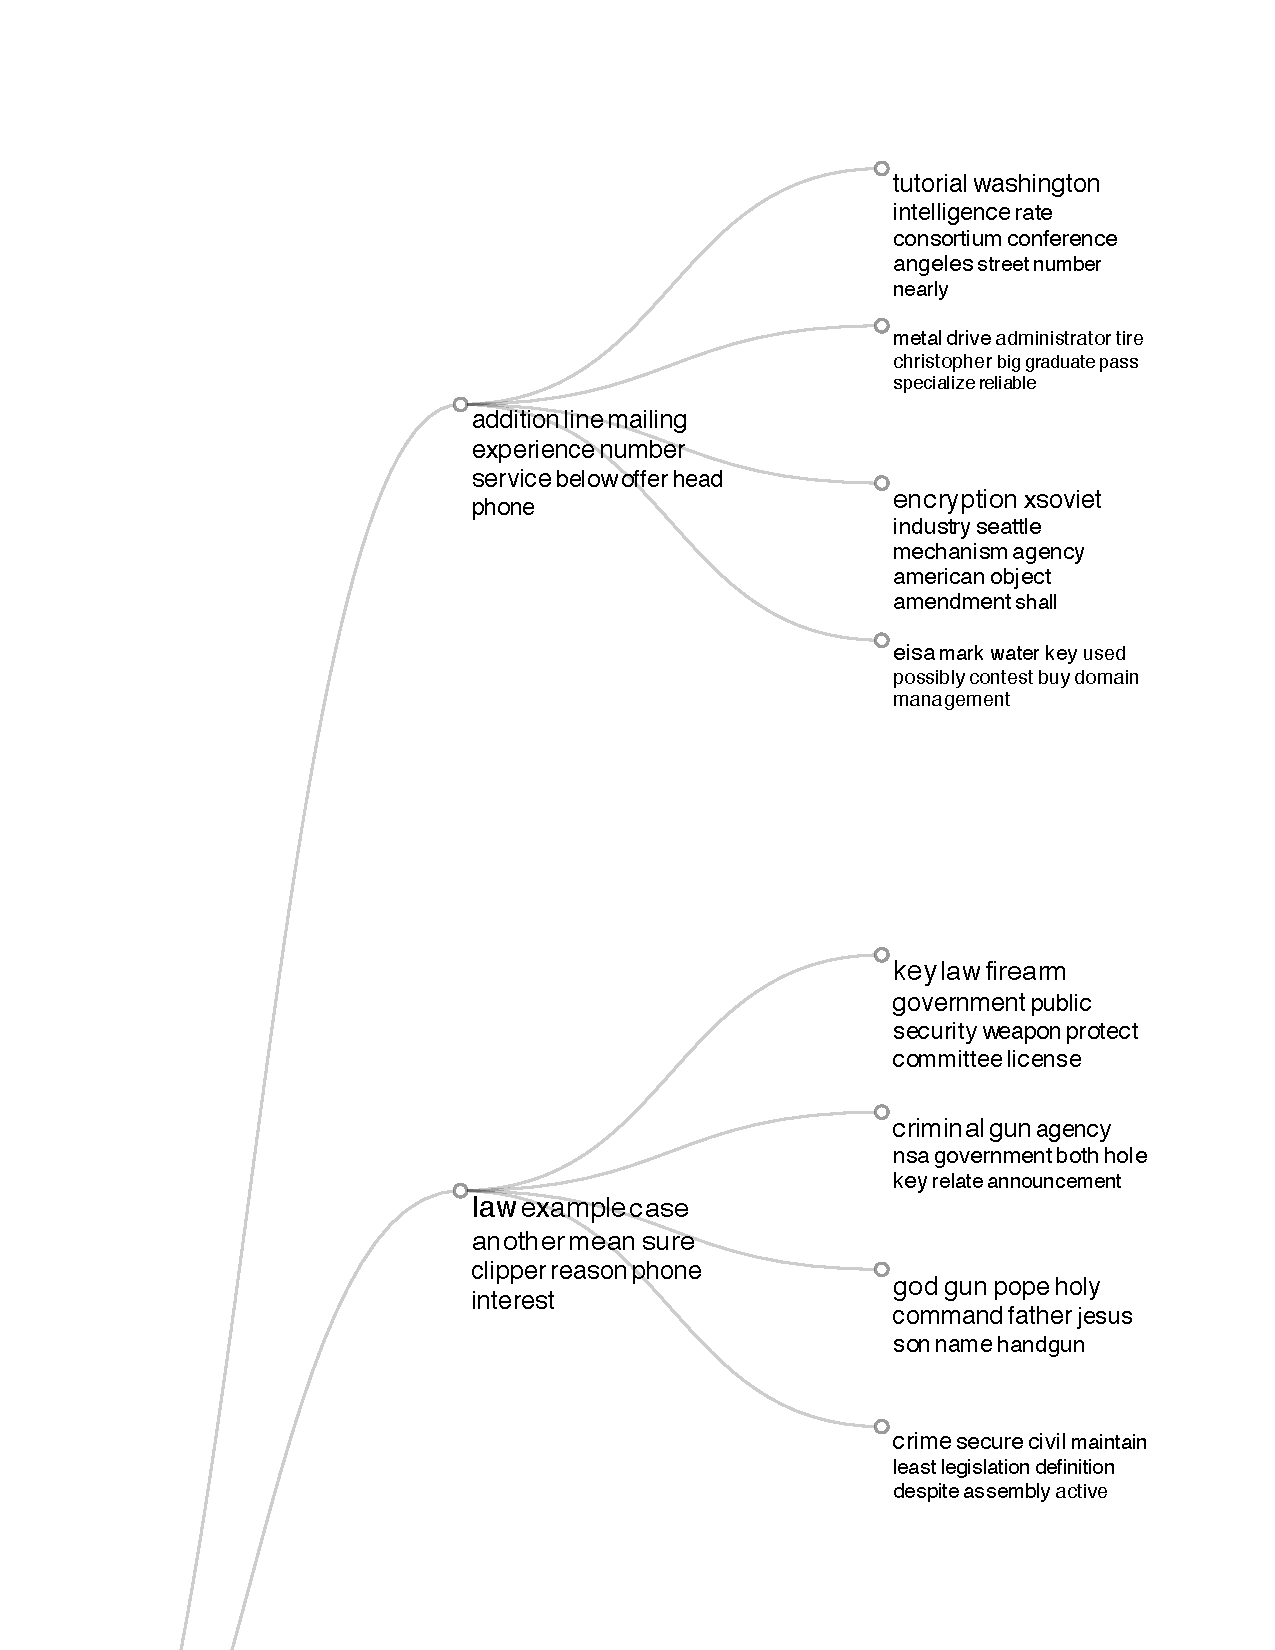
\includepdf[pages={-}]{graph.pdf}

Each document subtree can be visualized by drawing a copy of the global tree and highlighting the nodes selected for the given document.  If all subtrees are rendered at once there may be a heavy load on the renderer, so we implement a small amount of interactivity in order to only draw a few subtrees at a time.  The controls at the top of the following graphic are used to navigate between subtrees.

Note that it is not generally sensible to draw subtrees selected during the training procedure, as these are (generally) selected using different versions of the global parameters.  Additionally, if the subtrees and global tree are visualized simultaneously, many subtrees would be based on stale versions of the global parameters.  (In other words, we should only visualize test--time subtrees that are inferred using the same set of global parameters so that the nodes of one subtree represent the same topics as the nodes of another.)

Some ways we could augment the following visualization:
\begin{itemize}
\item Add tooltips or links from subtree nodes to global topics
\item Add a control (e.g., checkbox) to toggle displaying counts next to subtree nodes
\item Resize subtree nodes by absolute (global) weights (comparable between subtrees)
\item Color (e.g., heatmap, grayscale, opacity) subtree nodes by relative (per-document) weights (not comparable between subtrees, but would be expected to correlate with absolute weights); keep all edges black to retain clear indication of which nodes are actually selected
\end{itemize}

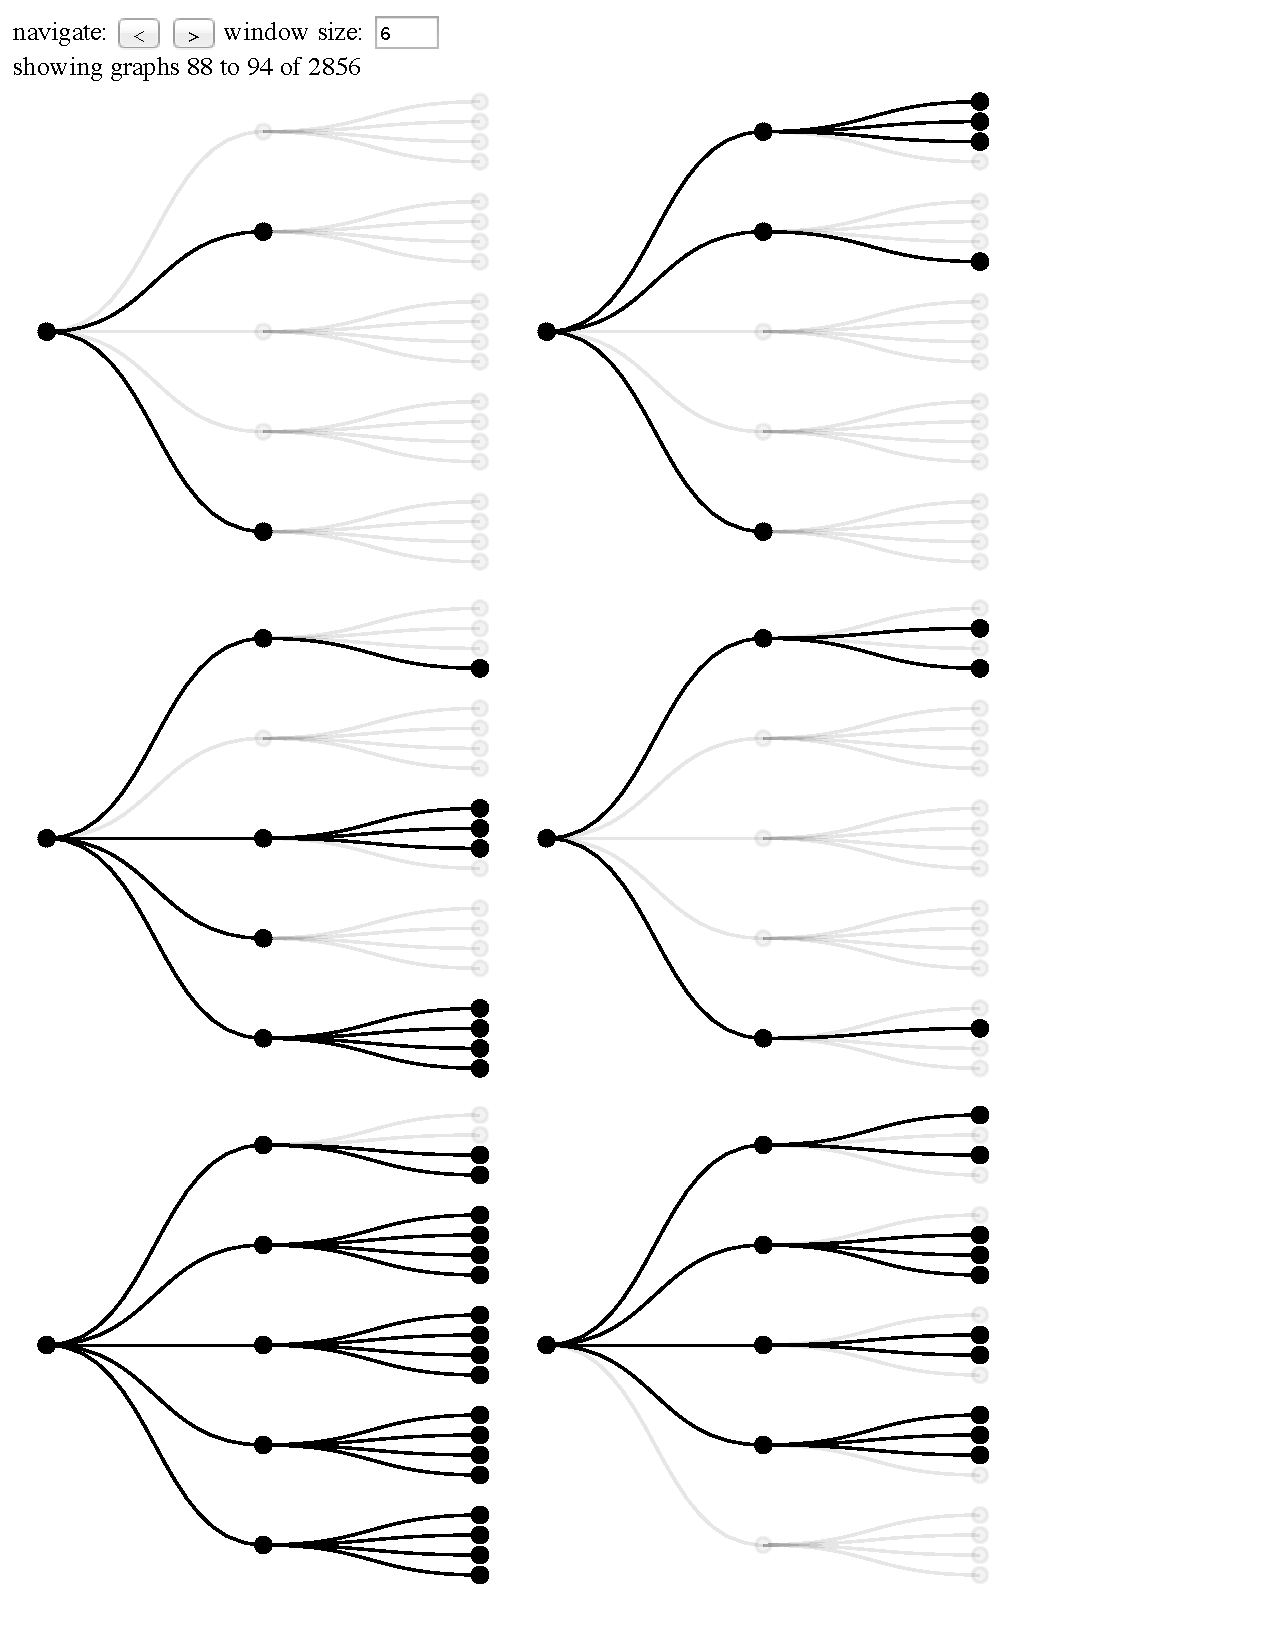
\includepdf[pages={-}]{subgraphs.pdf}




\section*{nHDP/nCRP hybrid personalized topic model (M1)}

\subsection*{True model}

In the generative story, we draw the global topics $\theta$ and stick-breaking weights $V_{\cdot}$, for each user we draw user-specific topics $\phi$ and stick-breaking weights $V_{\cdot}^{(u)}$, for each document of that user we draw a path $c_d^{(u)}$ from the tree and proportions over the levels $U'_{\cdot} \sim \GEM(m, \pi)$ (relative stick lengths $U_{\ell} \sim \Beta(m \pi, (1 - m) \pi)$ i.i.d.), and for each token in the document we draw a topic indicator $\zeta$ according to the level proportions $U$ and finally draw the word type $W$ from the corresponding $\phi$ (hence, $\theta$).  On the surface, the difference from the nHDP (M0), using the user--document metaphor, is that tokens for a user are drawn in a two-stage process from the local tree (the intermediate stage being documents), instead of being drawn directly from the local tree.

The distribution on the relative stick lengths can alternatively be parameterized as $\Beta(\gamma_1, \gamma_2)$, like the distribution on the local switching probabilities in M0.

The ELBO components for $\theta$, $V$, $V^{(u)}$, and $z^{(u)}$ do not change from M0.

The ELBO component for $c^{(u)}$ changes substantially; however, it can be easily deduced from the Beta formula.

TODO: we do not have hard assignments for any of the following, so... it is wrong:

The ELBO component for $U^{(u)}_d$ does not change in structure, however it is now computed within a user's document's path rather than within a document's tree.

The ELBO component for $\zeta^{(u)}_{dn}$ resembles the M0 ELBO component for $c_{dn}$.  The difference is that the prior $\pi^{(u)}_{di}$ is based only on $U^{(u)}_d$ and not $V^{(u)}$.

The ELBO component for $W^{(u)}_{dn}$

\ldots


\subsection*{Variational model}



\section*{HDP}



\section*{Supervised HDP (sHDP)}

\subsection*{True model}

\begin{itemize}
\item $\displaystyle H = \Dirichlet\left(\lambda_0 \one_\V\right)$ global distribution over words (cardinality $\V$)
\item $G \sim \DP\left(\alpha H\right)$ global topics
    \begin{itemize}
    \item $\theta_k \sim H$
    \item $V_k \sim \Beta(1, \alpha)$
    \end{itemize}
\item $p \sim \Dirichlet(\omega_0)$ class proportions
\item $G^{(m)} \sim \DP\left(\beta G\right)$ per-class topics
    \begin{itemize}
    \item $\theta_j^{(m)} \sim G$
    \item $V_j^{(m)} \sim \Beta(1, \beta)$
    \end{itemize}
\item $\Pr(y_j^{(m)} = k) = V_k \prod_{k'<k} (1 - V_{k'})$ class to global topic pointers
\item $x_d \sim \Discrete(p)$ observed document class
\item $G^{(d)} \sim \DP\left(\gamma G^{(m=x_d)}\right)$ per-document topics
    \begin{itemize}
    \item $\theta_i^{(d)} \sim G^{(m=x_d)}$
    \item $V_i^{(d)} \sim \Beta(1, \gamma)$
    \end{itemize}
\item $\Pr(z_i^{(d)} = j) = V_j^{(m=x_d)} \prod_{j'<j} (1 - V_{j'}^{(m=x_d)})$ document to class topic pointers
\item $\Pr(c_{dn} = i) = V_i^{(d)} \prod_{i'<i} (1 - V_{i'}^{(d)})$ topic assignments
\item $W_{dn} \sim \Discrete(W_{dn} \mid \theta_{y^{(x_d)}_{z^{(d)}_{c_{dn}}}})$ observed words
\end{itemize}


\subsection*{Variational model}

Global variables:
\begin{itemize}
\item $\displaystyle q(\theta_k) = \Dirichlet(\theta_k \mid \lambda_k)$
\item $\displaystyle q(V_k) = \Beta(V_k \mid \tau_k^{(1)}, \tau_k^{(1)})$
\item $q(p) = \Dirichlet(p \mid \omega)$
\end{itemize}
Class-wise variables:
\begin{itemize}
\item $\displaystyle q(V_j^{(m)}) = \Beta(V_j^{(m)} \mid a_j^{(m)}, b_j^{(m)})$
\item $q(y_j^{(m)}) = \Discrete(y_j^{(m)} \mid \psi_j^{(m)})$
\end{itemize}
Document-wise variables:
\begin{itemize}
\item $q(x_d) = \Discrete(x_d \mid \mu_d)$
\item $\displaystyle q(V_i^{(d)}) = \Beta(V_i^{(d)} \mid u_i^{(d)}, v_i^{(d)})$
\item $q(z_i^{(d)}) = \Discrete(z_i^{(d)} \mid \varphi_i^{(d)})$
\item $\displaystyle q(c_{dn}) = \Discrete(c_{dn} \mid \nu_{dn})$
\end{itemize}


\subsection*{ELBO}

\begin{align*}
\Lq
    &= \sum_k \left[ \Eq \log \Pr(V_k \mid \alpha) - \Eq \log q(V_k) \right] \\
    &\qquad + \sum_k \left[ \Eq \log \Pr(\theta_k \mid \lambda_0) - \Eq \log q(\theta_k) \right] \\
    &\qquad + \Eq \log \Pr(p \mid \omega_0) - \Eq \log q(p) \\
    &\qquad + \sum_{m,j} \left[ \Eq \log \Pr(V_j^{(m)} \mid \beta) - \Eq \log q(V_j^{(m)}) \right] \\
    &\qquad + \sum_{m,j} \left[ \Eq \log \Pr(y_j^{(m)} \mid V_\cdot) - \Eq \log q(y_j^{(m)}) \right] \\
    &\qquad + \sum_d \left[ \Eq \log \Pr(x_d \mid p) - \Eq \log q(x_d) \right] \\
    &\qquad + \sum_{d,i} \left[ \Eq \log \Pr(V_i^{(d)} \mid \gamma) - \Eq \log q(V_i^{(d)}) \right] \\
    &\qquad + \sum_{d,i} \left[ \Eq \log \Pr(z_i^{(d)} \mid V^{(m=\cdot)}_\cdot, x_d) - \Eq \log q(z_i^{(d)}) \right] \\
    &\qquad + \sum_{d,n} \left[ \Eq \log \Pr(c_{dn} \mid V^{(d)}_\cdot) - \Eq \log q(c_{dn}) \right] \\
    &\qquad + \sum_{d,n} \Eq \log \Pr(W_{dn} \mid c_{dn}, z_\cdot^{(d)}, x_d, y_\cdot^{(\cdot)}, \theta_{\cdot W_{dn}})
\end{align*}

We now derive components of the ELBO.

\begin{align*}
    &\Eq \log \Pr(V_k \mid \alpha) \\
    &= (\alpha - 1) \left[ \digamma{\tau_k^{(2)}} - \digamma{\tau_k^{(1)} + \tau_k^{(2)}} \right] - \log B(1, \alpha)
\end{align*}

\begin{align*}
    &\Eq \log q(V_k) \\
    &= (\tau_k^{(1)} - 1) \left[ \digamma{\tau_k^{(1)}} - \digamma{\tau_k^{(1)} + \tau_k^{(2)}} \right] \\
    &\qquad + (\tau_k^{(2)} - 1) \left[ \digamma{\tau_k^{(2)}} - \digamma{\tau_k^{(1)} + \tau_k^{(2)}} \right] \\
    &\qquad - \log B(\tau_k^{(1)}, \tau_k^{(2)})
\end{align*}

\begin{align*}
    &\Eq \log \Pr(\theta_k \mid \lambda_0) \\
    &= (\lambda_0 - 1) \sum_w \digamma{\lambda_{kw}} - W (\lambda_0 - 1) \digamma{\sum_w \lambda_{kw}} - \log B(\lambda_0 \one_W)
\end{align*}

\begin{align*}
    &\Eq \log q(\theta_k) \\
    &= \sum_w (\lambda_{kw} - 1) \digamma{\lambda_{kw}} - (\sum_w \lambda_{kw} - W) \digamma{\sum_w \lambda_{kw}} - \log B(\lambda_k)
\end{align*}

\begin{align*}
    &\Eq \log \Pr(p \mid \omega_0) \\
    &= (\omega_0 - 1) \sum_m \digamma{\omega_m} - M (\omega_0 - 1) \digamma{\sum_m \omega_m} - \log B(\omega_0 \one_M)
\end{align*}

\begin{align*}
    &\Eq \log q(p) \\
    &= \sum_m (\omega_m - 1) \digamma{\omega_m} - (\sum_m \omega_m - M) \digamma{\sum_m \omega_m} - \log B(\omega)
\end{align*}

\begin{align*}
    &\Eq \log \Pr(V_j^{(m)} \mid \beta) \\
    &= (\beta - 1) \left[ \digamma{b_j^{(m)}} - \digamma{a_j^{(m)} + b_j^{(m)}} \right] - \log B(1, \beta)
\end{align*}

\begin{align*}
    &\Eq \log q(V_j^{(m)}) \\
    &= (a_j^{(m)} - 1) \left[ \digamma{a_j^{(m)}} - \digamma{a_j^{(m)} + b_j^{(m)}} \right] \\
    &\qquad + (b_j^{(m)} - 1) \left[ \digamma{b_j^{(m)}} - \digamma{a_j^{(m)} + b_j^{(m)}} \right] \\
    &\qquad - \log B(a_j^{(m)}, b_j^{(m)})
\end{align*}

\begin{align*}
    &\Eq \log \Pr(y_j^{(m)} \mid V_\cdot) \\
    &= \sum_k \psi_j^{(m)}(k) \left[ \Eq \log V_k + \sum_{k'<k} \Eq \log (1-V_{k'}) \right]
\end{align*}

\begin{align*}
    &\Eq \log q(y_j^{(m)}) \\
    &= \sum_k \psi_j^{(m)}(k) \log \psi_j^{(m)}(k)
\end{align*}

\begin{align*}
    &\Eq \log \Pr(x_d \mid p) \\
    &= \sum_m \mu_{dm} \Eq \log p_m
\end{align*}

\begin{align*}
    &\Eq \log q(x_d) \\
    &= \sum_m \mu_{dm} \log \mu_{dm}
\end{align*}

\begin{align*}
    &\Eq \log \Pr(V_i^{(d)} \mid \gamma) \\
    &= (\gamma - 1) \left[ \digamma{v_i^{(d)}} - \digamma{u_i^{(d)} + v_i^{(d)}} \right] - \log B(1, \gamma)
\end{align*}

\begin{align*}
    &\Eq \log q(V_i^{(d)}) \\
    &= (u_i^{(d)} - 1) \left[ \digamma{u_i^{(d)}} - \digamma{u_i^{(d)} + v_i^{(d)}} \right] \\
    &\qquad + (v_i^{(d)} - 1) \left[ \digamma{v_i^{(d)}} - \digamma{u_i^{(d)} + v_i^{(d)}} \right] \\
    &\qquad - \log B(u_i^{(d)}, v_i^{(d)})
\end{align*}

\begin{align*}
    &\Eq \log \Pr(z_i^{(d)} \mid V^{(m=\cdot)}_\cdot, x_d) \\
    &= \sum_j \varphi_i^{(d)}(j) \left[ \sum_m \mu_{dm} \left[ \Eq \log V^{(m)}_j + \sum_{j'<j} \Eq \log (1-V^{(m)}_{j'}) \right] \right]
\end{align*}

\begin{align*}
    &\Eq \log q(z_i^{(d)}) \\
    &= \sum_j \varphi_i^{(d)}(j) \log \varphi_i^{(d)}(j)
\end{align*}

\begin{align*}
    &\Eq \log \Pr(c_{dn} \mid V^{(d)}_\cdot) \\
    &= \sum_i \nu_{dn}(i) \left[ \Eq \log V^{(d)}_i + \sum_{i'<i} \Eq \log (1-V^{(d)}_{i'}) \right]
\end{align*}

\begin{align*}
    &\Eq \log q(c_{dn}) \\
    &= \sum_i \nu_{dn}(i) \log \nu_{dn}(i)
\end{align*}

\begin{align*}
    &\Eq \log \Pr\left(W_{dn} \mid c_{dn}, z_\cdot^{(d)}, x_d, y_\cdot^{(\cdot)}, \theta_{\cdot W_{dn}}\right) \\
    &= \sum_i \nu_{dn}(i) \sum_j \varphi_i^{(d)}(j) \sum_m \mu_{dm} \sum_k \psi_j^{(m)}(k) \Eq \log \theta_{k W_{dn}}
\end{align*}

\subsection*{Coordinate ascent updates}

\begin{align*}
    &\pd{\tau_{k}^{(1)}} \Eq \left[ \log \Pr(V_k \mid \alpha) - \log q(V_k) + \sum_m \sum_j \log \Pr(y_j^{(m)} \mid V_\cdot) \right] \\
    &= (1 - \tau^{(1)}_k) \trigamma{\tau^{(1)}_k} - (1 + \alpha - \tau^{(1)}_k - \tau^{(2)}_k) \trigamma{\tau^{(1)}_k + \tau^{(2)}_k} \\
    &\qquad + \sum_m \sum_j \left[ \psi_j^{(m)}(k) \left[ \trigamma{\tau_{k}^{(1)}} - \trigamma{\tau_{k}^{(1)} + \tau_{k}^{(2)}} \right]
        - \sum_{k' > k} \psi_j^{(m)}(k') \trigamma{\tau_{k}^{(1)} + \tau_{k}^{(2)}} \right] \\
    &\Rightarrow
    \boxed{ \tau^{(1)}_k = 1 + \sum_m \sum_j \psi^{(m)}_j(k) }.
\end{align*}

\begin{align*}
    &\pd{\tau_{k}^{(2)}} \Eq \left[ \log \Pr(V_k \mid \alpha) - \log q(V_k) + \sum_m \sum_j \log \Pr(y_j^{(m)} \mid V_\cdot) \right] \\
    &= (\alpha - \tau^{(2)}_k) \trigamma{\tau^{(2)}_k} - (1 + \alpha - \tau^{(1)}_k - \tau^{(2)}_k) \trigamma{\tau^{(1)}_k + \tau^{(2)}_k} \\
    &\qquad + \sum_m \sum_j \left[ - \psi_j^{(m)}(k) \trigamma{\tau_{k}^{(1)} + \tau_{k}^{(2)}}
        + \sum_{k' > k} \psi_j^{(m)}(k') \left[ \trigamma{\tau_{k}^{(2)}} - \trigamma{\tau_{k}^{(1)} + \tau_{k}^{(2)}} \right] \right] \\
    &\Rightarrow
    \boxed{ \tau^{(2)}_k = \alpha + \sum_m \sum_j \sum_{k' > k} \psi^{(m)}_j(k') }.
\end{align*}

\begin{align*}
    &\pd{\lambda_{kw}} \Eq \left[ \log \Pr(\theta_k \mid \lambda_0) - \log q(\theta_k)
    + \sum_d \sum_n \Eq \log \Pr(W_{dn} \mid c_{dn}, z_\cdot^{(d)}, x_d, y_\cdot^{(\cdot)}, \theta_{k W_{dn}}) \right] \\
    &= (\lambda_0 - \lambda_{kw}) \trigamma{\lambda_{kw}} - \sum_{w'} (\lambda_0 - \lambda_{kw'}) \trigamma{\sum_{w''}{\lambda_{kw''}}} \\
    &\qquad + \sum_d \sum_n \delta_{W_{dn}}(w) \sum_i \nu_{dn}(i) \sum_j \varphi_i^{(d)}(j) \sum_m \mu_{dm} \psi_j^{(m)}(k) \left[ \trigamma{\lambda_{k w}} - \trigamma{\sum_{w'}{\lambda_{kw'}}} \right] \\
    &\Rightarrow
    \boxed{ \lambda_{kw} = \lambda_0 + \sum_d \sum_n \delta_{W_{dn}}(w) \sum_i \nu_{dn}(i) \sum_j \varphi_i^{(d)}(j) \sum_m \mu_{dm} \psi_j^{(m)} }.
\end{align*}

\begin{align*}
    &\pd{\omega_m} \Eq \left[ \log \Pr(p \mid \omega_0) - \log q(p) + \sum_d \log \Pr(x_d \mid p) \right] \\
    &= (\omega_0 - \omega_m) \trigamma{\omega_m} - \trigamma{\sum_{m'} \omega_{m'}} \sum_{m'} (\omega_0 - \omega_{m'}) \\
    &\qquad + \sum_d \left[ \mu_{dm} \trigamma{\omega_m} - \trigamma{\sum_{m'} \omega_{m'}} \sum_{m'} \mu_{dm'} \right] \\
    &\Rightarrow
    \boxed{ \omega_m = \sum_m \mu_{dm} }.
\end{align*}

\begin{align*}
    &\pd{a_j^{(m)}} \Eq \left[ \log \Pr(V_j^{(m)} \mid \beta) - \log q(V_j^{(m)}) + \sum_d \sum_i \log \Pr(z_i^{(d)} \mid V^{(m=\cdot)}_\cdot, x_d) \right] \\
    &= (1 - a_j^{(m)}) \trigamma{a_j^{(m)}} - (1 + \beta - a_j^{(m)} - b_j^{(m)}) \trigamma{a_j^{(m)} + b_j^{(m)}} \\
    &\qquad + \sum_d \mu_{dm} \sum_i \left[ \varphi_i^{(d)}(j) \left[ \trigamma{a_j^{(m)}} - \trigamma{a_j^{(m)} + b_j^{(m)}} \right] - \sum_{j'>j} \varphi_i^{(d)}(j') \trigamma{a_j^{(m)} + b_j^{(m)}} \right] \\
    &\Rightarrow
    \boxed{ a_j^{(m)} = 1 + \sum_d \mu_{dm} \sum_i \varphi_i^{(d)}(j) }.
\end{align*}

\begin{align*}
    &\pd{b_j^{(m)}} \Eq \left[ \log \Pr(V_j^{(m)} \mid \beta) - \log q(V_j^{(m)}) + \sum_d \sum_i \log \Pr(z_i^{(d)} \mid V^{(m=\cdot)}_\cdot, x_d) \right] \\
    &= (\beta - b_j^{(m)}) \trigamma{b_j^{(m)}} - (1 + \beta - a_j^{(m)} - b_j^{(m)}) \trigamma{a_j^{(m)} + b_j^{(m)}} \\
    &\qquad + \sum_d \mu_{dm} \sum_i \left[ - \varphi_i^{(d)}(j) \trigamma{a_j^{(m)} + b_j^{(m)}} + \sum_{j'>j} \varphi_i^{(d)}(j') \left[ \trigamma{b_j^{(m)}} + \trigamma{a_j^{(m)} + b_j^{(m)}} \right] \right] \\
    &\Rightarrow
    \boxed{ b_j^{(m)} = \beta + \sum_d \mu_{dm} \sum_i \sum_{j' > j} \varphi_i^{(d)}(j') }.
\end{align*}

\begin{align*}
    &\pd{\psi_j^{(m)}} \Eq \left[ \log \Pr(y_j^{(m)} \mid V_\cdot) - \log q(y_j^{(m)}) + \sum_d \sum_n \log \Pr\left(W_{dn} \mid c_{dn}, z_\cdot^{(d)}, x_d, y_\cdot^{(\cdot)}, \theta_{\cdot W_{dn}}\right) \right] \\
    &= \sum_k \left[ \Eq \log V_k + \sum_{k'<k} \Eq \log (1-V_{k'}) + \sum_d \mu_{dm} \sum_n \sum_i \nu_{dn}(i) \varphi_i^{(d)}(j) \Eq \log \theta_{k W_{dn}} \right] \\
    &\qquad - \sum_k \left[ 1 + \log \psi_j^{(m)}(k) \right] \\
    &\Rightarrow
    \boxed{ \psi_j^{(m)}(k) \propto \exp\left[ \Eq \log V_k + \sum_{k'<k} \Eq \log (1-V_{k'}) + \sum_d \mu_{dm} \sum_n \sum_i \nu_{dn}(i) \varphi_i^{(d)}(j) \Eq \log \theta_{k W_{dn}} \right] } .
\end{align*}

\begin{align*}
    &\pd{\mu_{d\cdot}} \Eq \left[ \log \Pr(x_d \mid p) - \log q(x_d) + \sum_d \sum_i \log \Pr(z_i^{(d)} \mid V^{(m=\cdot)}_\cdot, x_d) \right] \\
    &= \sum_m \left[ \Eq \log{p_m} + \sum_d \sum_i \sum_j \varphi_i^{(d)}(j) \left[ \Eq \log V^{(m)}_j + \sum_{j'<j} \Eq \log (1-V^{(m)}_{j'}) \right] \right] \\
    &\qquad - \sum_m \left[ 1 + \log \mu_{dm} \right] \\
    &\Rightarrow
    \boxed{ \mu_{dm} \propto \exp\left[ \Eq \log{p_m} + \sum_d \sum_i \sum_j \varphi_i^{(d)}(j) \left[ \Eq \log V^{(m)}_j + \sum_{j'<j} \Eq \log (1-V^{(m)}_{j'}) \right] \right] }.
\end{align*}

\begin{align*}
    &\pd{u_i^{(d)}} \Eq \left[ \log \Pr(V_i^{(d)} \mid \gamma) - \log q(V_i^{(d)}) + \sum_n \log \Pr(c_{dn} \mid V^{(d)}_\cdot) \right] \\
    &= (1 - u_i^{(d)}) \trigamma{u_i^{(d)}} - (1 + \gamma - u_i^{(d)} - v_i^{(d)}) \trigamma{u_i^{(d)} + v_i^{(d)}} \\
    &\qquad + \sum_n \left[ \nu_{dn}(i) \left[ \trigamma{u_i^{(d)}} - \trigamma{u_i^{(d)} + v_i^{(d)}} \right] - \sum_{i'>i} \nu_{dn}(i') \trigamma{u_i^{(d)} + v_i^{(d)}} \right] \\
    &\Rightarrow
    \boxed{ u_i^{(d)} = 1 + \sum_n \nu_{dn}(i) }.
\end{align*}

\begin{align*}
    &\pd{v_i^{(d)}} \Eq \left[ \log \Pr(V_i^{(d)} \mid \gamma) - \log q(V_i^{(d)}) + \sum_n \log \Pr(c_{dn} \mid V^{(d)}_\cdot) \right] \\
    &= (\gamma - v_i^{(d)}) \trigamma{v_i^{(d)}} - (1 + \gamma - u_i^{(d)} - v_i^{(d)}) \trigamma{u_i^{(d)} + v_i^{(d)}} \\
    &\qquad + \sum_n \left[ - \nu_{dn}(i) \trigamma{u_i^{(d)} + v_i^{(d)}} + \sum_{i'>i} \nu_{dn}(i') \left[ \trigamma{v_i^{(d)}} - \trigamma{u_i^{(d)} + v_i^{(d)}} \right] \right] \\
    &\Rightarrow
    \boxed{ v_i^{(d)} = 1 + \sum_n \sum_{i'>i} \nu_{dn}(i') }.
\end{align*}

\begin{align*}
    &\pd{\varphi_i^{(d)}} \Eq \left[ \log \Pr(z_i^{(d)} \mid V^{(m=\cdot)}_\cdot, x_d) - \log q(z_i^{(d)}) + \sum_n \log \Pr\left(W_{dn} \mid c_{dn}, z_\cdot^{(d)}, x_d, y_\cdot^{(\cdot)}, \theta_{\cdot W_{dn}}\right) \right] \\
    &= \sum_j \sum_m \mu_{dm} \left[ \Eq \log V_j^{(m)} + \sum_{j'<j} \Eq \log (1-V_{j'}^{(m)}) + \sum_n \nu_{dn}(i) \sum_k \psi_j^{(m)}(k) \Eq \log \theta_{k W_{dn}} \right] \\
    &\qquad - \sum_j \left[ 1 + \log \varphi_i^{(d)}(j) \right] \\
    &\Rightarrow
    \boxed{ \varphi_i^{(d)}(j) \propto \exp\left[ \sum_m \mu_{dm} \left[ \Eq \log V_j^{(m)} + \sum_{j'<j} \Eq \log (1-V_{j'}^{(m)}) + \sum_n \nu_{dn}(i) \sum_k \psi_j^{(m)}(k) \Eq \log \theta_{k W_{dn}} \right] \right] } .
\end{align*}

\begin{align*}
    &\pd{\nu_{dn}} \Eq \left[ \log \Pr(c_{dn} \mid V^{(d)}_\cdot) - \log q(c_{dn}) + \log \Pr\left(W_{dn} \mid c_{dn}, z_\cdot^{(d)}, x_d, y_\cdot^{(\cdot)}, \theta_{\cdot W_{dn}}\right) \right] \\
    &= \sum_i \left[ \Eq \log V_i^{(d)} + \sum_{i'<i} \Eq \log (1-V_{i'}^{(d)}) + \sum_j \varphi_i^{(d)}(j) \sum_m \mu_{dm} \sum_k \psi_j^{(m)}(k) \Eq \log \theta_{k W_{dn}} \right] \\
    &\qquad - \sum_i \left[ 1 + \log \nu_{dn}(i) \right] \\
    &\Rightarrow
    \boxed{ \nu_{dn}(i) \propto \exp\left[ \Eq \log V_i^{(d)} + \sum_{i'<i} \Eq \log (1-V_{i'}^{(d)}) + \sum_j \varphi_i^{(d)}(j) \sum_m \mu_{dm} \sum_k \psi_j^{(m)}(k) \Eq \log \theta_{k W_{dn}} \right] } .
\end{align*}



\section*{Joint hierarchical geolocation-language models}

There are a number of ways to formulate a joint model of geolocation and language based on the nHDP.  The first, M2, comes from prior work under the nCRF moniker \cite{ahmed2013,ahmed2013a}.  However, the attribute cascade makes this model a challenge for inference.

\subsection*{nCRF model with flat global topics, attribute cascade (M2)}

\subsubsection*{True model}

In the nHDP, each document is a tree drawn using the global tree as a base distribution; in particular, each document defines a distribution over nodes and each word in a given document is assigned a topic according to that document's distribution.  In the joint model (nCRF application), each user is a tree (drawn using the global tree as a base distribution) and each document emitted by that user is allocated one of the nodes (joint geolocation-language variables) according to the user's distribution over nodes.  In the nHDP, each node in the global tree is endowed with a topic; in the nCRF, each node in the global tree is endowed with a mean location, regional topic, and topic distribution.

Specifically, instead of just endowing each node with a topic $\theta$ (locally: $\phi$), we endow each node with a mean location $\mu$, regional topic $\phi$, and topic proportion vector $\theta$ (locally: same variable name with a superscript $(d)$).  Note, the local attributes are just copies of global attributes, but the indices are permuted due to exchangeability(?) in the stick-breaking construction.  This is in contrast to nHDP, in which

However, whereas in nHDP we draw $\theta$ from $G_0$ i.i.d., in the nCRF we want to cascade $\mu$, $\phi$, and $\theta$ down the (global) tree, i.e.\ we want to draw $\mu_{i_\ell,j}$ from $\Normal(\mu_{i_\ell}, \Sigma_{i_\ell})$, draw $\phi_{i_\ell,j}$ from $\Dirichlet(\omega \phi_{i_\ell})$, and draw $\theta_{i_\ell,j}$ from $\Dirichlet(\lambda \theta_{i_\ell})$.

Is there a similar discrepancy in the local node attributes?  It seems in the nCRF each node in a user's tree corresponds directly to a node in the global tree.  Does the nHDP have the same configuration?  Specifically, are the attributes (topics) of the children of a given node simply permuted in the document trees, or are they actually drawn from the global distribution, so that two children of the node may be endowed with the same topic?  (I suspect the latter.)

In the nHDP we draw the atoms of a node in a document's tree i.i.d.\ from the parent node (a DP).  In the nCRF, in contrast,

\ldots


\subsubsection*{Variational model}



\bibliographystyle{plain}
\bibliography{notes}

\end{document}
